\documentclass[tikz, border = 5pt]{standalone}
\usepackage{tikz}

\usetikzlibrary{arrows.meta}
\usetikzlibrary{shapes.geometric}

\begin{document}

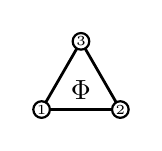
\begin{tikzpicture}[scale = 1.0]

	% model Parameters
	\def \base{2}	% number of sites in base
	\def \a{1}	% lattice paramters

	% artistic parameters
	\def \lw{1pt}
	\def \circsize{3pt}

	% get physical coordiantes of points from i and j
	\newcommand{\getpoint}[2]{%
    		\pgfmathsetmacro{\X}{\a*(#1-0.5*#2)}%
    		\pgfmathsetmacro{\Y}{\a*#2*sqrt(3)/2}%
	}


	
	% Create lattice points 
	\foreach \i in {1,...,\base}{
		\foreach \j in {1,...,\i}{
			\getpoint{\i}{\j}
			\coordinate (P-\i-\j) at (\X, \Y);
		}
	}
	

	% Draw nearest neighbour links
	\foreach \i in {1,...,\base}{
		\foreach \j in {1,...,\i}{
				
			% to right and top right:
			\ifnum \i < \base 
				\draw[line width = \lw] (P-\i-\j) -- (P-\the\numexpr\i+1\relax-\j);
				\draw[line width = \lw] (P-\i-\j) -- (P-\the\numexpr\i+1\relax-\the\numexpr\j+1\relax);
			\fi

			% to top left 
			\ifnum \j < \i
				\draw[line width = \lw] (P-\i-\j) -- (P-\i-\the\numexpr\j+1\relax);
			\fi	
		}
	}
	
	% bubbles at lattice points with site numbers
	
	\filldraw[color = black, fill = white, thick] (P-1-1) circle (\circsize);
	\node[font = \tiny] at (P-1-1) {1};
	\filldraw[color = black, fill = white, thick] (P-2-1) circle (\circsize);
	\node[font = \tiny] at (P-2-1) {2};
	\filldraw[color = black, fill = white, thick] (P-2-2) circle (\circsize);
	\node[font = \tiny] at (P-2-2) {3};

	
	% Phi in the middle of rectangle

	\pgfmathsetmacro{\midX}{\a}
	\pgfmathsetmacro{\midY}{\a*6*3*sqrt(3)/(4*7)}

	\node at (\a, \midY) {$\Phi$};
\end{tikzpicture}

\end{document}
